\input{head.inc}

% Präambelbefehle für die Präsentation
\title[TET: Magnetostatik II - Materie]{Magnetostatik II - Materie}

\begin{document}
% 
% Frontmatter 
% 
%%%%%%%%%%%%%%%%%%%%%%%%%%%%%%%%%%%%%%%%%%%%%%%%%%%%%%%%%%%%%%%%%%%%%%%%%%%%%%%%%%%%%%%%%%%%%%%%%%%%%%%%%%%%%%%%%%%%%%%%%%%%% 

%% inserts the title page and the table of contents
\maketitle

% 
% Content 
% 
%%%%%%%%%%%%%%%%%%%%%%%%%%%%%%%%%%%%%%%%%%%%%%%%%%%%%%%%%%%%%%%%%%%%%%%%%%%%%%%%%%%%%%%%%%%%%%%%%%%%%%%%%%%%%%%%%%%%%%%%%%%%% 
\section{Magnetostatik II - Materie}

\begin{frame}

  \frametitle{Mikroskopische vs makroskopische Betrachtung}

  \begin{itemize}[<+->]
  \item Wie bereits in \enquote{Elektrostatik VIII - Materie} diskutiert und erläutert: Die Maxwell-Gleichungen des Vakuums gelten auch in Materie.
  \item Allerdings müssten dann die \alert{Bewegungen aller Ladungsträger} betrachtet werden, die aber nur zu einem Bruchteil zu einer \alert{makroskopischen Stromdichte} beiträgt. $\to$ Makroskopische Betrachtung im Sinne von Mittelwerten.
    \item Analog zur elektrischen Flussdichte \(\verschiebung[v] \) mit
$\verschiebung[v] = \varepsilon_0 \efeld[v] + \vec{P}$
folgt für das Magnetfeld in Materie unter Einführung der \alert{Magnetisierung} \(\magnetis[v] \)
\begin{align*}
	& \boxed{\magfeld[v] = \dfrac{1}{\mu_0} \tetB[v] - \magnetis[v]}
		&& \Leftrightarrow
		&&	\boxed{\tetB[v] = \mu_0  \left( \magfeld[v] + \magnetis[v] \right)}
\end{align*}
\item In der Maxwellgleichung $\rotation \magfeld[v] = \elstromdichte[v]$
ist $\elstromdichte[v]$ als \alert{makroskopisch gemittelte Stromdichte} zu verstehen.
\item Für ein \alert{lineares, isotropes und homogenes Medium} kann mit Hilfe der \alert{magnetischen Suszeptibilität} \(\chi_\mathrm{m} \) gilt für die Magnetisierung:$\boxed{\magnetis[v] = \chi_\mathrm{m}  \magfeld[v]}$
\item Damit folgt für die magnetische Permeabilität:
$\boxed{\mu_\mathrm{r} = 1 + \chi_\mathrm{m} }$
\item Somit ergibt sich für die magnetische Induktion:
$\boxed{\tetB[v] = \left( 1 + \chi_\mathrm{m} \right) \mu_0 \magfeld[v]
		= \mu_0 \mu_\mathrm{r} \magfeld[v] }$
\end{itemize}
\end{frame}

\begin{frame}
  \frametitle{Einteilung der magnetischen Materie}
  \begin{itemize}[<+->]
  \item \alert{Diamagnetismus:}
    \begin{itemize}[<+->]
    \item Diamagnetismus ist eine Eigenschaft \alert{aller Stoffe}, kann aber von anderen Eigenschaften überlagert werden.
    \item Keine permanente interne magnetische Dipole.
    \item Induzierte Magnetisierung im äußeren Feld $\to$ wirkt seiner Ursache entgehen
    \item Es gilt $\chi_\mathrm{m} < 0$ und $|\chi_\mathrm{m}| \simeq 10^{-5}$
    \item Spezialfall \alert{Supraleiter} $\to$ Meißner-Ochsenfeld-Effekt (komplette Feldverdrängung)
      $\chi_\mathrm{m} = -1 \quad \text{ perfekter Diamagnetismus}$
      \end{itemize}
  \item \alert{Paramagnetismus:}
    \begin{itemize}[<+->]
    \item Es gibt \alert{permanente interne magnetische Dipole}, die sich im äußeren Feld orientieren können.
    \item Die thermische Bewegung wirkt der Ordnung entgegen.
    \item Daher gilt allgemein: $\chi_\mathrm{m} > 0 \text{ und } \chi_\mathrm{m} = \chi_\mathrm{m}(T)$
    \item Je nach Ursache des Paramagnetismus (gebundene Elektronen vs. freie Leitungselektronen) ist die magnetische Suszeptibilität entweder \alert{temperaturabhängig} (gebundene Elektronen) oder (fast) \alert{temperaturunabhängig} (Leitungselektronen $\to$ \alert{Pauli-Paramagnetismus}).
    \item Im Falle der Temperaturabhängigkeit gilt (zumindest bei ausreichend hohen Temperaturen) das \alert{Curie-Gesetz} $\chi_\mathrm{m}(T) = \frac{C}{T}$
      \end{itemize}
\end{itemize}
\end{frame}


\begin{frame}
  \frametitle{Einteilung der magnetischen Materie (fortgesetzt)}
  \begin{itemize}[<+->]
    \item \alert{Kollektiver Magnetismus} $\to$ Ferro-, Ferri-, Antiferromagnetismus
    \begin{itemize}[<+->]
    \item Es gibt \alert{permanente interne magnetische Dipole}, die sich im äußeren Feld orientieren können.
    \item Die thermische Bewegung wirkt der Ordnung entgegen.
      \item Aber: Unterhalb einer kritischen Temperatur $T^\star$ kommt es durch eine (quantenmechanische) \alert{Austauschwechselwirkung} auch ohne äußeres Feld zu einer \alert{spontanen Ausrichtung}.
    \item Die Suszeptibilität ist häufig eine komplizierte Funktion (mindestens) von Feld und Temperatur:
      $$
      \chi_\mathrm{m} = \chi_\mathrm{m}(T, H, \dots)
      $$
      \item Der kollektive Magnetismus gliedert sich in Ferro-, Ferri- und Antiferromagnetismus
      \end{itemize}
\end{itemize}
\end{frame}


\begin{frame}
  \frametitle{Ferromagnetismus - wichtig: Fe, Co, Ni}
  \begin{itemize}[<+->]
  \item $T=0$: Alle permanente magnetische Dipole gleich ausgerichtet
  \item $0<T\le T^\star=T_C$ \alert{(Curie-Temperatur)}: zunehmende Unordnung durch thermische Bewegung
  \item $T>T_C$: normaler Paramagnetismus
    \item typisch für ferromagnetische Stoffe:
  \begin{itemize}[<+->]
  \item $\chi_m > 0$ und $|\chi_m|$ sehr groß (1.000, 10.000, 100.000)
    \item Hysterese
    \item Weißsche Bezirke: Ursache für Hysterese
  \end{itemize}
\end{itemize}\pause
\resizebox{.4\linewidth}{!}{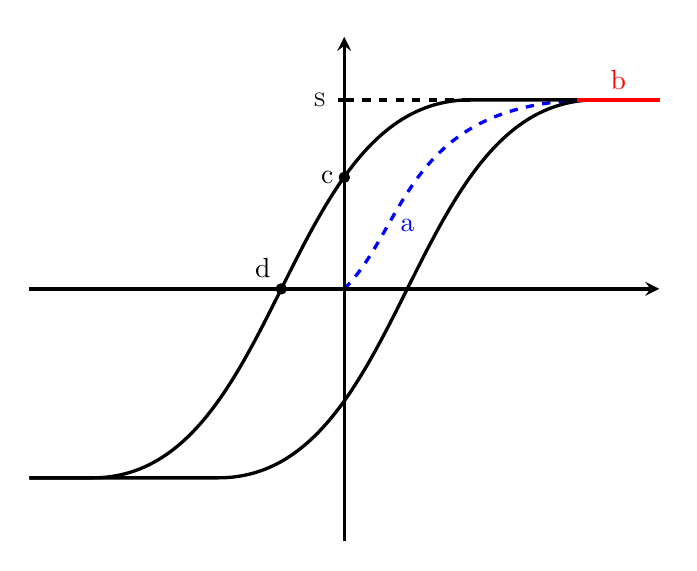
\begin{tikzpicture}[line width = 1.2pt, line join=round,x=1cm,y=1cm,>=stealth, scale = 0.8]
	% Neukurve
	\draw [dashed, color=blue] (0,0) to [controls={+(1,1) and +(-3,0)}] (4,3) -- (5,3);
	% Koordinatensystem
	\draw [->] (-5,0) -- (5,0) node [anchor = north] {$ \HFeld $};
	\draw [->] (0,-4) -- (0,4) node [anchor = east] {$ \Magnetisierung $};
	% Sättigungs Magnetisierung
	\draw [dashed] (2,3) -- (0,3);
	\draw (0.1,3) -- (-0.1,3) node[anchor=east] {$ \Magnetisierung_\mathrm{S} $};
	% Hysteresekurve
	\draw (-5,-3) -- (-4,-3) to [controls={+(3,0) and +(-3,0)}] (2,3) -- (5,3);
	\draw (5,3) -- (4,3) to [controls={+(-3,0) and +(3,0)}] (-2,-3) -- (-5,-3);
	% Erläuterungen
	\draw [color=blue] (1,1) node {a};
	\draw [color=red] (3.7,3) -- (5,3) node [anchor=south,midway] {b};
	\filldraw (0,1.77) circle (1.8pt) node [anchor = east] {c};
	\filldraw (-1,0) circle (1.8pt) node [anchor=south east] {d};
\end{tikzpicture}}\hspace*{1cm}\resizebox{.4\linewidth}{!}{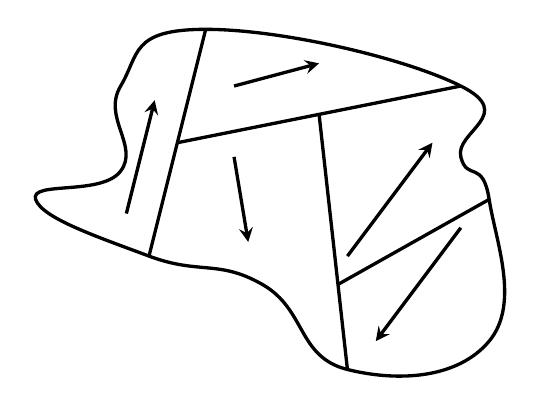
\begin{tikzpicture}[line width = 1.2pt, line join=round,x=0.4cm,y=0.4cm,>=stealth, scale=0.9]
	\coordinate (a) at (0,0);
	\coordinate (b) at (4,-1);
	\coordinate (c) at (7,-4);
	\coordinate (d) at (12,-3);
	\coordinate (e) at (12,2);
	\coordinate (f) at (11,3.5);
	\coordinate (g) at (11,6);
	\coordinate (h) at (2,8);
	\coordinate (i) at (-1,6);
	\coordinate (j) at (-1,3);
	\coordinate (k) at (-4,2);
	% Zwischenpunkte (halbe Strecken meist
	\coordinate (ah) at (1,4);
	\coordinate (ahg) at (6,5);
	% 1/3
	\coordinate (ahgi) at ({6+2/3},-1);
	% Rahmen
	\draw plot [smooth cycle, tension=0.8] coordinates {(a) (b) (c) (d) (e) (f) (g) (h) (i) (j) (k)};
	% Trennlinien
	\draw (a) -- (h);
	\draw (ah) -- (g);
	\draw (ahg) -- (c);
	\draw (ahgi) -- (e);
	% Pfeile
	\draw [->] (-0.8,1.5) -- ++(1,4);
	\draw [->] (3,6) -- ++(3,0.8);
	\draw [->] (3,3.5) -- ++(0.5,-3);
	\draw [->] (7,0) -- ++(3,4);
	\draw [->] (11,1) -- ++(-3,-4);
\end{tikzpicture}}
\end{frame}

\begin{frame}
  \frametitle{Ferri- und Antiferromagnetismus}
  \begin{itemize}[<+->]
  \item Ferrimagnetismus:
  \begin{itemize}[<+->]
  \item Festkörper setzt sich aus zwei Untergittern zusammen
  \item Beide sind jeweils ferromagnetisch
    \item Aber die jeweilige Magnetisierung ist nicht gleich und kompensiert sich teilweise.
  \end{itemize}
  \item Antiferromagnetismus:
  \begin{itemize}[<+->]
  \item Spezialfall der Ferrimagnetismus
  \item Beide Untergitter gleich stark magnetisiert. Aber umgekehrte Richtung.
  \item Kritische Temperatur heißt hier \alert{N{\'e}el-Temperatur}
  \item Unterhalb: keine Magnetisierung
    \item Oberhalb: Paramagnetismus (aber: $\chi_m=\chi_m(H)$) 
  \end{itemize}
\end{itemize}
\end{frame}



\begin{frame}
  \frametitle{Randwertaufgaben - magnetische Skalarpotential}
  \begin{itemize}[<+->]
  \item Einfachster Fall: lineares, isotropes, homogenes Medium im \alert{gesamten} Lösungsvolumen: $\laplace \magvekpot[v]= -\mu \elstromdichte[v](\ortsvektor[v])$ $\to$ Lösungsmethoden bekannt
  \item Auch einfach: \alert{bereichsweise} lineare, isotrope, homogene Medien im Lösungsvolumen: Lösung in jedem Teilbereich, freie Konstanten so anpassen, dass Stetigkeitsbedingungen erfüllt werden.
  \item Keine Ströme im Lösungsvolumen $V$ und Randwerte auf $O(V)$:
      \begin{itemize}[<+->]
      \item In V: $\rotation\magfeld[v] = \vec{0}$
        $$
        \magfeld[v](\ortsvektor[v]) = -\gradient \phi_m (\ortsvektor[v]) \quad \text{\alert{magnetisches Skalarpotential }} \phi_m (\ortsvektor[v]) 
        $$
      \item Mit zumindest bereichsweise konstanten $\mu_r$ folgt:
        $$
        \divergenz \tetB[v] = 0 = \divergenz \left[\mu_0\mu_r \left(-\gradient \phi_m \right)\right] \Rightarrow \boxed{\laplace \phi_m = 0}
        $$
        \item Aus der Elektrostatik bekannte Lösungsmethoden mit Berücksichtigung der vorgegebenen Randbedingungen anwenden.
\end{itemize}
\end{itemize}
\end{frame}

\begin{frame}
  \frametitle{Randwertaufgaben - magnetische Skalarpotential}
  \begin{itemize}[<+->]
  \item Keine Ströme im Lösungsvolumen $V$ und Randwerte auf $O(V)$; \alert{zusätzlich:} $\vec{M}(\ortsvektor[v])\ne \vec{0}$ in $V$:
      \begin{itemize}[<+->]
      \item In V: $\rotation\magfeld[v] = \vec{0}$
        $$
        \magfeld[v](\ortsvektor[v]) = -\gradient \phi_m (\ortsvektor[v]) 
        $$
      \item Mit zumindest bereichsweise konstanten $\mu_r$ folgt:
        $$
        \divergenz \tetB[v] = 0 = \mu_0\divergenz ( \underbrace{-\gradient \phi_m }_{\magfeld[v]}+\vec{M}) \Rightarrow \boxed{\laplace \phi_m = \divergenz \vec{M}} \text{ Poisson-Gleichung}
        $$
      \item Ohne Randbedingungen folgt damit:
        $$
        \phi_m (\ortsvektor[v]) = -\frac{1}{4\pi} \int \frac{\divergenz \vec{M} (\ortsvektor[vs]) }{|\ortsvektor[v]-\ortsvektor[vs]|} \upd V'
        $$
        \item Mit Randbedingungen (Dirichlet: $\phi_m$ auf dem Rand gegeben; Neumann: $\frac{\partial\phi_m}{\partial n} = \vec{n}\cdot\gradient\phi_m = - \vec{n}\cdot\magfeld[v]$ auf dem Rand gegeben) $\to$ Lösungsmethoden für Poisson-Gleichung mit Randbedingungen anwenden.
\end{itemize}
\end{itemize}
\end{frame}



\input{finalframe.inc}
   
\end{document}